\documentclass[12pt,a4paper]{article}
\usepackage[
	left 	= 2.5cm,
	right 	= 2.5cm, 
	top 		= 2.5cm,
	bottom 	= 2.5cm,
]{geometry}
\usepackage[utf8]{inputenc}
\usepackage[english]{babel}
\usepackage[OT1]{fontenc}
\usepackage{amsmath}
\usepackage{mathtools}
\usepackage{graphicx}
\usepackage{caption}
\usepackage[round]{natbib}

\usepackage[hidelinks]{hyperref}
\hypersetup{
	colorlinks = true,
	urlcolor   = blue,
	linkcolor  = black, 
	citecolor  = blue, 
}


\usepackage{fancyhdr}
\pagestyle{fancy}
\lhead{\slshape Unterweger, Oberbrinkmann \& Lohre}
\chead{}
\rhead{\slshape \nouppercase{\leftmark}}

\usepackage{titlesec,xcolor}
\titleformat{\section}{\bfseries}{\thesection}{0.5em}{}
\titlespacing{\section}{0pt}{3ex plus 1ex minus 0.2ex}{10pt}
\setlength{\headheight}{14.49998pt}

\usepackage{titlesec,xcolor}
\titleformat{\subsection}{\bfseries}{\thesubsection}{0.5em}{}
\titlespacing{\subsection}{0pt}{3ex plus 1ex minus 0.2ex}{10pt}
\setlength{\headheight}{14.49998pt}


%------------------------------------------------------------------%

\author{Lucas Paul Unterweger, Sophia Oberbrinkmann, Fynn Lohre}
\title{The Kremlin Effect: How Geographical Proximity to Russia Affects Military Spending}


\begin{document}

\begin{titlepage}
\center
\vfill

\includegraphics[scale=0.08]{WU.png}
\vfill
\begin{tabular}[t]{lc}
Course:  & Advanced Macroeconometrics (Science Track) \\
Examiner: & 
Nikolas Kuschnig, MSc (WU) \& Lukas Vashold, MSc (WU) \\
Submission date: & 31.07.2023 \\
\end{tabular}
\vfill
{\large \textbf{The Kremlin Effect: How Geographical Proximity to Russia Affects Military Spending}}
\vfill
by\\ \vspace{3mm}
{\Large Lucas Unterweger \href{https://github.com/therealLucasPaul}{
\includegraphics[scale=0.01]{GitHub.png}}}\\
(Matr.-Nr. h11913169 )\\ \vspace{3mm}
\& \\ \vspace{3mm}
{\Large Sophia Oberbrinkmann \href{https://github.com/SophiaOberbrinkmann}{
\includegraphics[scale=0.01]{GitHub.png}}}\\
(Matr.-Nr. h12225352)\\ \vspace{3mm}
\& \\ \vspace{3mm}
{\Large Fynn Lohre \href{https://github.com/VARFynn}{
\includegraphics[scale=0.01]{GitHub.png}}}\\
(Matr.-Nr. h12232560)\
\vfill

\thispagestyle{empty}
\pagebreak
\end{titlepage}
\newcounter{savepage}
\pagenumbering{roman}
\thispagestyle{empty}
\begin{abstract}
\textit{We present a study on how the distance of a country’s capital to Moscow affects its military spending. To tackle the research question, we combine different datasets from various sources, such as the SIPRI Military Expenditure Database, the GeoDist database, and the Electoral Democracy Index. A Bayesian Model Averaging (BMA) approach is used to account for model uncertainty and estimate several models with different distance measures and covariates. Our results identify a in terms of posterior model probability superior model and show that the capital distance to Moscow has a significant negative effect on military expenditures, implying that countries closer to Russia perceive a higher threat and allocate more resources to defense. Additionally, it's observable that continents play a pivotal role in explaining the variation in military expenditures. Specifically a general underestimation of possible threats in Europe is indicated. The effects of border degree and democracy index as additional layers of distance are mixed and remain to some extend uncertain.} 
\end{abstract}
\clearpage
\thispagestyle{plain}
\tableofcontents
\pagebreak
\setcounter{savepage}{\arabic{page}}
\pagenumbering{arabic}
\section{Introduction}
Our research project delves into the intriguing question of whether the distance of a country's capital to Moscow has a significant impact on its military spending. To tackle this question, we employ a Bayesian regression analysis.

Our research is inspired and built upon the insights provided by two seminal papers: the work of \citet{kofrovn2023} and \citet{nordhaus2012}. \citet{kofrovn2023} focused on the Russo-Ukrainian conflict's impact on the military expenditures of European States. They made a thought-provoking observation, suggesting that physical geography continues to play a pivotal role in shaping military affairs and geopolitics, even in the 21st century. On the other hand, Nordhaus, and his coauthors (\citeyear{nordhaus2012}) investigated how a country's external security environment influences its military spending. Their extensive analysis, covering 165 countries from 1950 to 2000, demonstrated that the prospectively generated estimate of the external threat served as a potent variable in explaining military expenditures. Drawing upon these foundational ideas, our research seeks to utilize the geographical distance to Russia, as highlighted by \citet{kofrovn2023}, as a proxy for external threat, echoing Nordhaus's emphasis. To justify this assumption, we consider the historical background of Russia and the Soviet Union. Given that the NATO was established as a response to the perceived political aggression of the Soviet Union during the Cold War, and it currently comprises 31 member states, it reinforces our belief that Russia is often seen as a potential threat.

While our focus centers on the geographical distance to Russia as an external factor influencing military expenditure, we recognize that numerous other determinants have been extensively analyzed. A plethora of authors have shed light on different potential causes, broadly categorized into external factors (such as military expenditures of potential enemies or allies, and perceived threats) and internal influences, encompassing economic, political, and bureaucratic factors \citep{nikolaidou2008}. The research results across various studies, some conducted on individual countries while others on groups of countries or spanning the entire globe \citep{nikolaidou2008,george2018,nordhaus2012}, have yielded somewhat ambiguous findings \citep{nikolaidou2008,odehnal2020}. 
Given the relative dearth of studies exploring the specific influence of geographical distance to Russia on military spending \citep{kofrovn2023}, we aim to contribute to the existing literature by focusing on this understudied factor. Our expectation is that a closer distance to Russia would be positively correlated with increased military expenditure by the concerned country.  

As part of our investigation, we also consider the NATO member countries, who are expected to allocate 2 \% of their annual GDP to military expenditures uniformly. Any deviation from this standard percentage rate could further strengthen our hypothesis regarding the role of geographical distance to Russia in a country's military spending decision. Furthermore, we expand our analysis beyond NATO members to include non-NATO countries, recognizing that recent events like the Russo-Ukraine conflict highlight Russia's perceived threat by countries worldwide. Our study encompasses a total of 151 countries, offering a comprehensive global perspective. 

To gauge the geographical distance to Russia, we explore various approaches, evaluating how the estimation may be influenced by these different measures. Our primary proxies are the capital distances of countries measured in kilometers, as this offers a relevant metric for military threats. While \citet{kofrovn2023} considered road travel distance and mention the potential of flight travel distance, we prioritize air distance as a more appropriate proxy when examining military threats. 
In our pursuit of a comprehensive and nuanced analysis, we recognize that relying solely on the distance between capitals might not fully capture the complex dynamics and interactions between countries. Therefore, we go beyond the capital distance and incorporate a second measure — the border degree of a country with Russia — to gain deeper insights into the relationship between geographical proximity and military expenditure decisions. The border degree metric enables us to examine how the presence of a common border with Russia, or even a second-degree border (i.e., sharing a border with a country that shares a border with Russia), may exert distinct influences on a country's military spending compared to the air distance metric. By exploring the border degree, we aim to understand whether physical contiguity with Russia plays a unique role in shaping a country's perception of threats and security concerns, and consequently, its military expenditure decisions. Countries sharing a direct border with Russia may experience more immediate security considerations, influenced by historical conflicts, geopolitical tensions, or territorial disputes. On the other hand, second-degree border countries might have indirect security implications resulting from their proximity to nations with a direct border with Russia. These indirect influences might manifest in different ways and warrant closer examination.

Moving forward, our research report will be structured as follows: we will first delve into the \textit{Data} we utilize, emphasizing its relevance and reliability. Subsequently, we will detail the \textit{Econometric Framework}, with particular emphasis on our novel approach of employing Bayesian Model Averaging, a technique not previously utilized in the papers we draw inspiration from. We will then present the \textit{Results} of our investigation, providing insights into the potential relationships uncovered, before we analyze the results and prevailing limitations in the \textit{Discussion}. Finally, we will conclude the project with a comprehensive \emph{Summary},
highlighting the implications of our findings and potential avenues for further research.

%\clearpage
%\section{Literature Review}
%\clearpage
\section{Data}
In order to provide an answer to our research question, it is necessary to combine different datasets. These different sets of data are (i) the \citet{SIRPI} by the Stockholm International Peace Research Institute Stockholm International Peace Research Institute (SIRPI), (ii) the GeoDist database provided by the Centre d'Etudes Prospectives et d'Informations Internationales (CEPII; \citealp{mayer2011}) and (iii) the electoral democracy index based on the Varieties of Democracy (V-Dem) dataset \citep{VDEM} by the Department of Political Science located at the University of Gothenburg. 

The SIRPI database contains consistent time series on the military spending of 173  countries for the period 1949–2022 and, hence, represents our essential measurement for a country's military expenditure, namely \textit{''Military Expenditure by Country as percentage of GDP"}. Their definition of military expenditure includes all spending on current military forces and activities, meaning the armed forces, including peace keeping forces; defense ministries and other government agencies engaged in defense projects; paramilitary forces when judged to be trained, equipped and available for military operations; and military space activities. With respect to the reliability of the data, it should still be noted that the data collected is not only derived from primary sources, but also includes secondary sources and estimates, e.g. from the IMF or NATO.
 
\pagebreak
The CEPII database includes an exhaustive set of gravity variables and, thus, a bilateral measurement of distance, namely distance the capital city in each country (\textit{''Distance''}). Although the data set had originally been created for a 2005 paper, it has no bearing on reliability, as changes in city distance are either zero or if at all marginal. In addition, we manually checked the distance for randomly drawn distance pairs.

The Electoral Democracy Index (\textit{''V-Dem Index''}) classifies countries as being more or less democratic  on a scale zero to one and is our approach to not only capture geographical but also structural sociological differences. The resulting democratic distance is the difference between a country's and Russia's assigned value. The respective value stems from the consultation of almost 4000 ''experts'' within the scope of the V-Dem project. Although an attempt within the V-Dem project is made to select as diverse a sample of individuals, with respect to reliability, it cannot be ruled out that the index is affected by an Educational- or Western-bias.

Additionally, we manually create the following variables \textit{''Direct Border''} and \textit{''Secondary Border''}, capturing the existence of a direct border and a border with a state with a direct border, respectively; \textit{''NATO''}, a dummy for a NATO membership; \textit{''OKVS''}, a dummy for a Collective Security Treaty Organization membership;\textit{''BRICS''}, a dummy for a BRICS membership and \textit{''Neutrality''}, a dummy capturing the political Neutrality in Austria and Switzerland. 


This leads to our final dataset which contains 151 countries after removing countries, which do not exist anymore, as well as Russia, Kosovo and South Sudan.\footnote{Russia for plausibility reasons	and Kosovo/South Sudan for lacking data.} \hyperref[t:1]{\color{blue} Table 1} allows to derive our core data structure for the given time stamp 2021.


\begin{table}[h]
\label{t:1}
\caption{Summary Statistics of Key Variables for t = 2021}
\begin{tabular}{lrrrrrr}
\hline \hline
Variable & N & Mean & Std. Dev. & Min. & Max. \\ \hline
Military Expenditure as \% of GDP & 151 & 1.82 & 1.32 & 0.11 & 7.58 \\
Distance &   151  &  5,912.68 &   3,711.31 & 686.96 &  16,774.49 \\
V-Dem Index & 149 & 0.54& 0.25 & 0.02 & 0.92 \\
Direct Border & 151 & 0.10 & 0.30 & 0.00 & 1.00 \\
Secondary Border & 151 & 0.13 & 0.34 & 0.00 &          1.00 \\
NATO & 151& 0.20 & 0.40 & 0.00 & 1.00 \\         
OKVS & 151 & 0.03  & 0.17 & 0.00 & 1.00 \\
BRICS & 151  & 0.03 & 0.16 & 0.00 & 1.00 \\          
Neutrality & 151   &  0.01 &   0.11 & 0.00 & 1.00 \\     \hline\hline
\end{tabular}
\end{table}
 
\section{Econometric Framework}
In order to draw inference, but also reflect existing model uncertainty, we use Bayesian Model Averaging (BMA) as our approach to tackle the underlying research question.  Instead of just estimating one model $\hat{M}$ and updating our prior beliefs $p(\theta)$ to posterior beliefs $p(\theta \vert data)$, we estimate several models $M_{i}$ incorporating different distance measures and covariates. Afterwards, we take the combined parameter distribution, weighted by the posterior model probability of all candidate models to draw conclusions (i.e. BMA; following \citealp{jeffreys1939} and \citealp{jevons1874}). The used posterior model probability reflects the plausibility of a model given the data, i.e. $p(M_{i} \vert data)$.
\clearpage 
Applied to our research question, namely whether distance to Russia (or Moskow) is a predictor of military expenditure, this implies that we first have to define the candidate models, reflecting our uncertainty about the different layers of distance. Given the heterogeneity of data availability, we first estimate the models for 2021 and, afterwards, use different time settings as robustness-checks. Thus, the model specifications are as follows: 
\begin{align}
 M_1 \coloneqq \textrm{2021 Military Expenditure} \sim \textrm{Distance} + \textrm{V-Dem Index} + \textrm{Direct Border} \\ +  \textrm{ Secondary Border} +  \textrm{NATO} + \textrm{OKVS} + \textrm{BRICS} + \textrm{Neutrality} \nonumber
\end{align}\\[-3.1em]
\begin{align}
 M_2 \coloneqq \textrm{2021 Military Expenditure} \sim \textrm{Distance} + \textrm{Direct Border} + \textrm{Secondary Border} \\ + \textrm{ NATO} + \textrm{OKVS} + \textrm{BRICS} + \textrm{Neutrality} \nonumber
\end{align}\\[-3.1em]
\begin{align}
M_3 \coloneqq \textrm{2021 Military Expenditure} \sim \textrm{Distance} 
\end{align}\\[-3.1em]
\begin{align}
  M_4 \coloneqq \textrm{2021 Military Expenditure} \sim \textrm{Direct Border} + \textrm{Secondary Border} \\ + \textrm{ NATO} + \textrm{OKVS} + \textrm{BRICS} + \textrm{Neutrality} \nonumber
\end{align}
We fit these Bayesian regression models using a Markov Chain Monte Carlo (MCMC) algorithm to obtain posterior distributions for the model parameters. The MCMC sampling includes two chains and a total of 1000 iterations, with the first 500 iterations discarded as burn-in period to ensure convergence. In order to be non-influential, allowing the data to have a dominant role in the estimation of model parameters, we use weakly uninformative priors, namely a normal distribution with mean 0 and standard deviation 1 for the regression coefficients and an inverse gamma distribution with shape parameter 2 and scale parameter 1 for the error's term standard deviation.
\begin{figure}[h]
\center
\label{F:1}
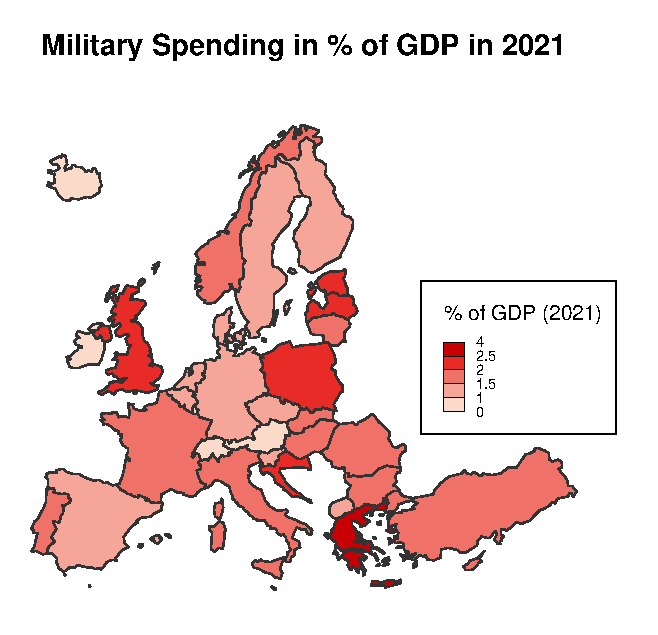
\includegraphics[scale=0.75]{Map1.pdf}
\caption{Mapped Military Expenditure for Europe in 2021}
\end{figure}
\section{Results}
Looking at the mapped military expenditures in 2021 for Europe (see \hyperref[F:1]{\color{blue}Figure 1}), a slight trend in the descriptive data is evident, indicating that, with the exception of the UK, military expenditures are higher for countries closer to Russia. It also seems that the degree of border also positively (captured in the following regressions through \textit{''Direct Border''} and \textit{''Secondary Border''}) correlates with higher military expenditures. 

\clearpage
\begin{figure}
\center
\label{F:2}
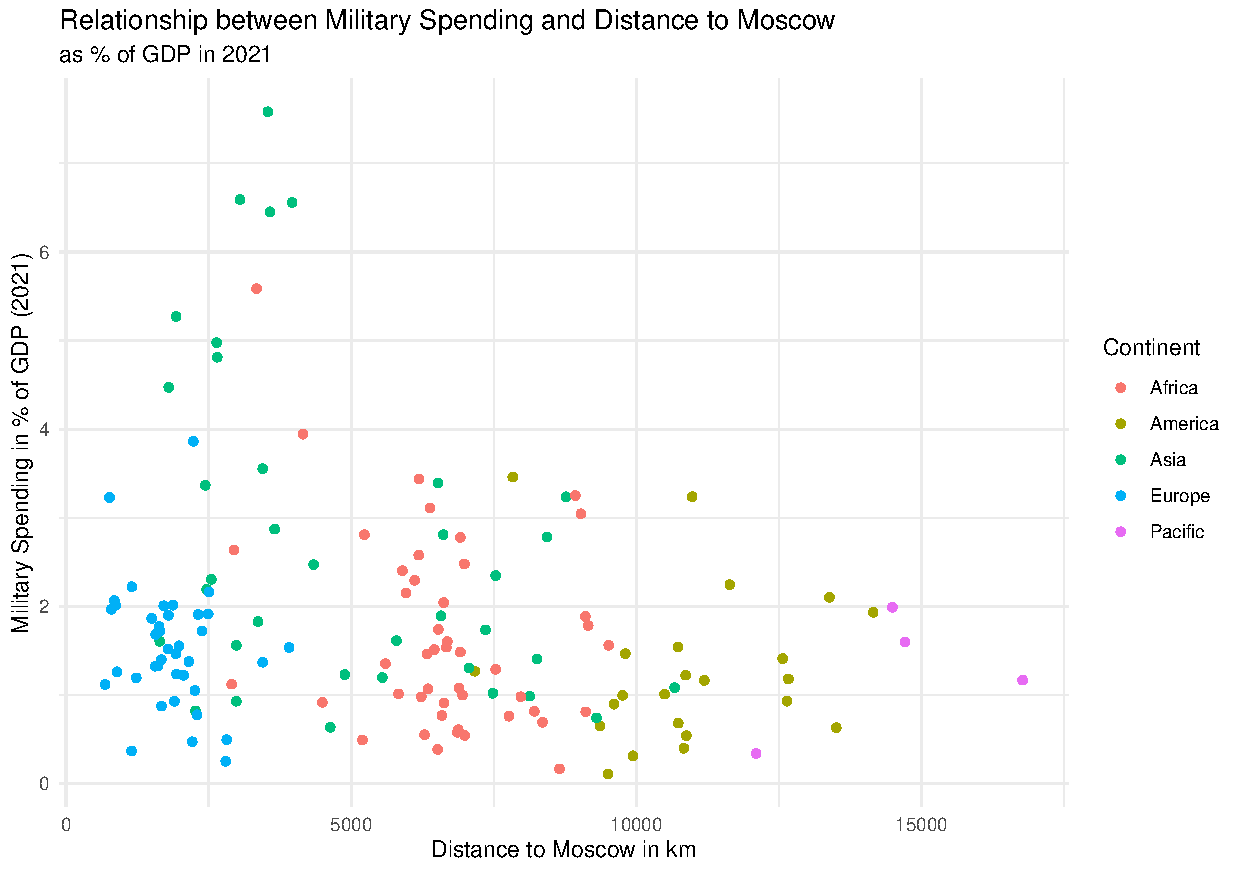
\includegraphics[scale=0.36]{Plot2.pdf}
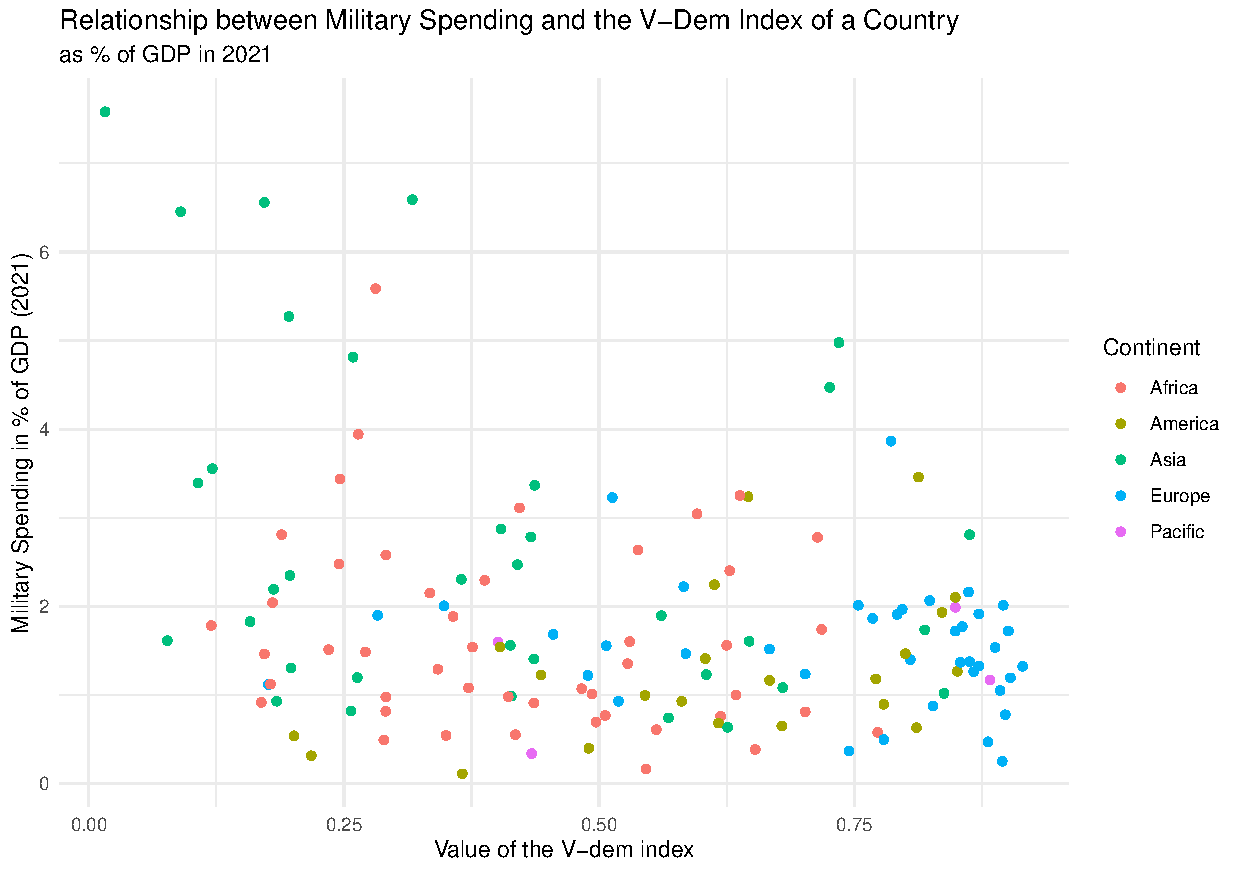
\includegraphics[scale=0.36]{Plot3.pdf}
\caption{Relationship between Military Expenditure and Distance to Moscow as well as V-Dem Index of a Country in 2021}
\end{figure}

Extending the descriptive visualization to the entire data set in form of a scatter-plot (see \hyperref[F:2]{\color{blue}Figure 2, left panel}) again shows a first indication that the distance to Moscow - and, thus, Russia - may affect a country's military expenditure, as the variance decreases if the distance increases. Yet, one can at the same time see the respective continent as well influencing the relationship. Looking at the scatter-plot (see \hyperref[F:2]{\color{blue}Figure 2, right panel}) visualizing a possible linkage between military expenditures and the V-Dem index, as a proxy for sociological distance, a clear effect is not visible.  Instead, a correlation between the continent and the extend of democracy is observable. Thus, a sociological distance might be to some extend captured in a possible effect by the continents. These purely descriptive relationships are now to be verified within the framework of the Bayesian model estimations carried out.  


\begin{table}[!htbp] \centering 
  \caption{Estimates of $M_1$, Bayesian Regression for t = 2021} 
  \label{T:2} 
\begin{tabular}{@{\extracolsep{5pt}} ccccc} 
\\[-1.8ex]\hline 
\hline \\[-1.8ex] 
\textit{Military Expenditure in \% of GDP} & Estimate & Est.Error & Q2.5 & Q97.5 \\ 
\hline \\[-1.8ex] 
Intercept & $3.259$ & $0.394$ & $2.475$ & $4.012$ \\ 
Distance & $$-$0.0002$ & $0.0001$ & $$-$0.0003$ & $$-$0.0001$ \\ 
Nato & $0.402$ & $0.357$ & $$-$0.283$ & $1.083$ \\ 
BRICS & $$-$0.303$ & $0.545$ & $$-$1.391$ & $0.772$ \\ 
OKVS & $$-$0.780$ & $0.503$ & $$-$1.722$ & $0.230$ \\ 
America & $0.522$ & $0.356$ & $$-$0.166$ & $1.182$ \\ 
Asia & $0.952$ & $0.274$ & $0.435$ & $1.507$ \\ 
Europe & $$-$1.038$ & $0.421$ & $$-$1.850$ & $$-$0.228$ \\ 
Pacific & $1.127$ & $0.617$ & $0.026$ & $2.330$ \\ 
Direct Border & $$-$0.334$ & $0.345$ & $$-$0.974$ & $0.336$ \\ 
Secondary Border & $$-$0.469$ & $0.310$ & $$-$1.078$ & $0.147$ \\ 
V-Dem Index & $$-$0.488$ & $0.454$ & $$-$1.422$ & $0.435$ \\ 
\hline \hline \\[-1.8ex] 
\end{tabular} 
\end{table} 


\hyperref[T:2]{\color{blue}Table 2} shows the estimates of the first model, $M_1$, including all covariates. The estimated interval for \textit{Distance} ranges from $-0.00034$ to $-0.00012$, implying that a 1,000 km higher distance induces a decrease in \textit{Military Expenditure} between $0.34$ and $0.12$ percentage points. The subsequent posterior distribution for the parameter \textit{Distance} is shown in \hyperref[F:3]{\color{blue}Figure 3} and highlights the exclusion of zero in the estimated interval. Moreover, it appears that a higher sociological distance to Russia (with a V-Dem rating of $0.22$) and a higher level of democracy may lead to lower \textit{Military Expenditures} (estimated interval $-1.422$ \& $0.435$). However, it is especially visible in the posterior distribution of the respective parameter, that there is no clear evidence for a negative effect. It is also visible that the estimated intervals for the continents include higher absolute values while also excluding zero (only exception is \textit{America}). Interestingly, $M_1$ suggests a first indication of a negative effect for a \textit{Direct} ($-0.974$ \& $0.336$ as interval) and \textit{Secondary Border }($-1.078$ \& $0.147$).



\begin{figure}[t]
\center
\label{F:3}
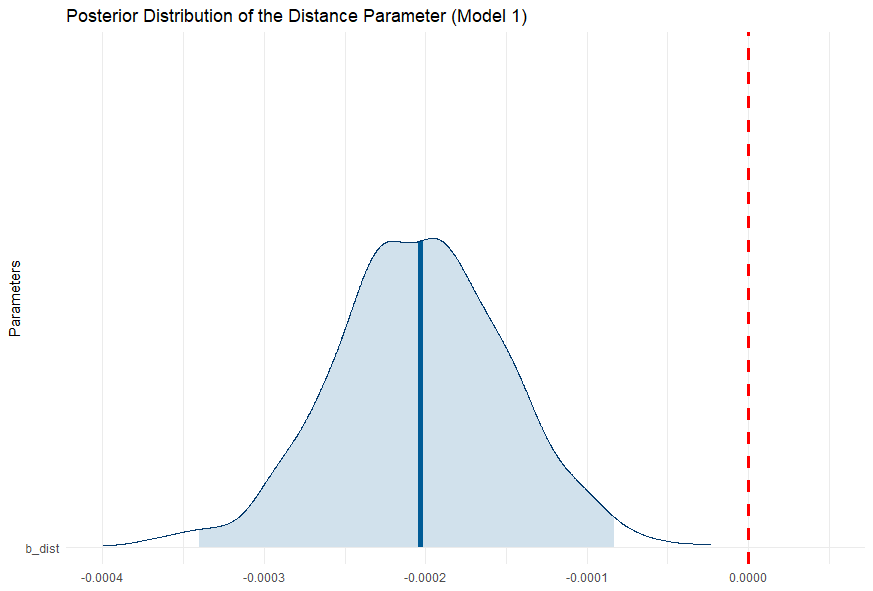
\includegraphics[scale=0.25]{PosteriorPlot_Distance_Model1.png}
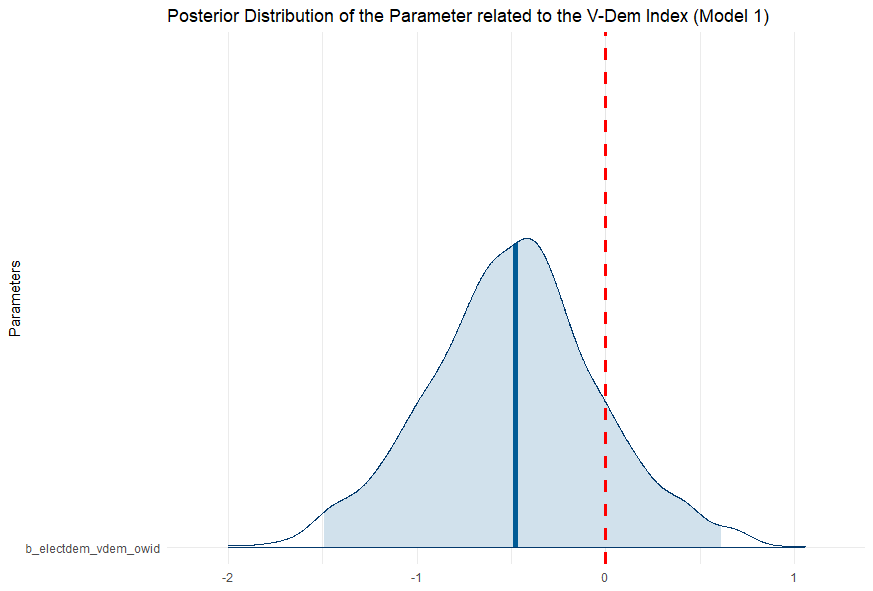
\includegraphics[scale=0.25]{PosteriorPlot_VDem_Model1.png}
\caption{Posterior Distributions $M_1$, Distance and V-Dem Index}
\end{figure}

\begin{figure}[h]
\center
\label{F:4}
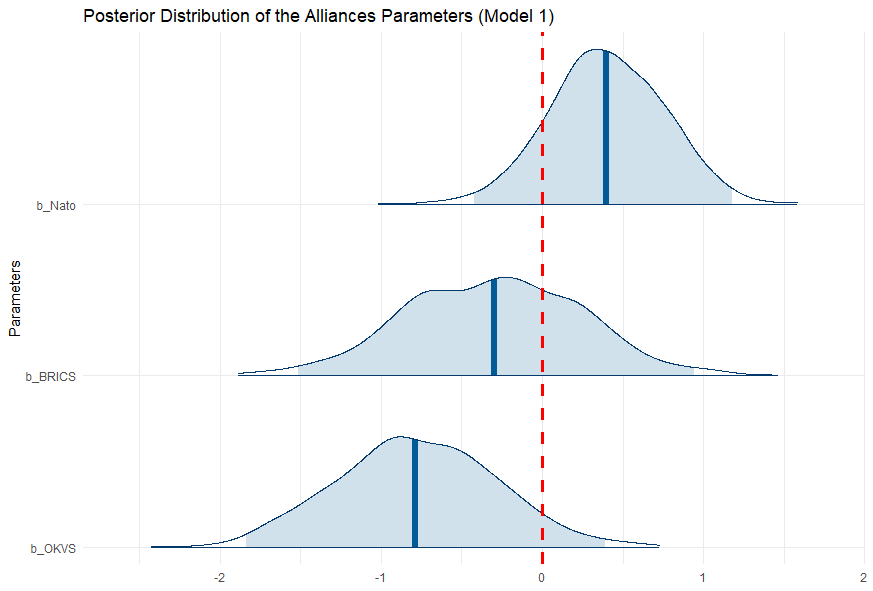
\includegraphics[scale=0.2]{PosteriorPlot_Alliances_Model1.png}
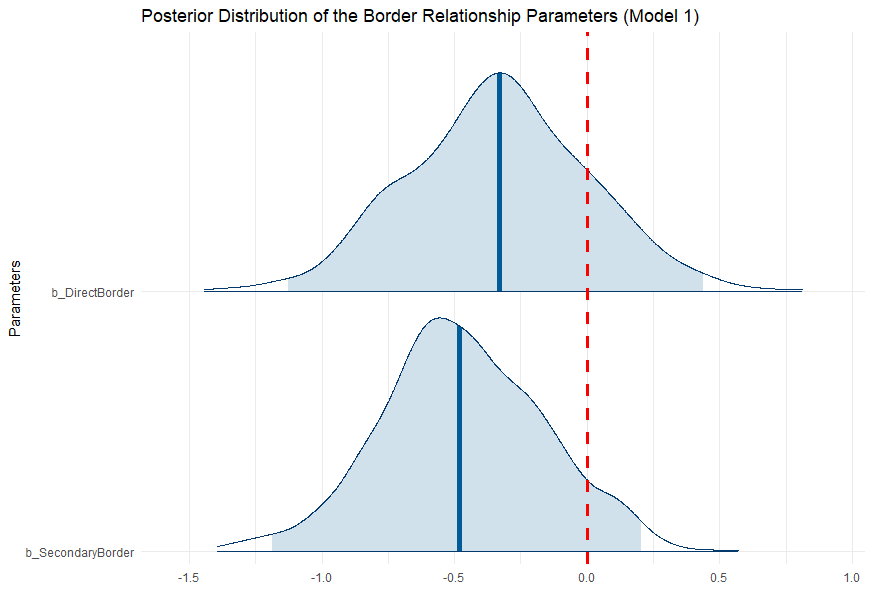
\includegraphics[scale=0.2]{PosteriorPlot_Border_Model1.png}
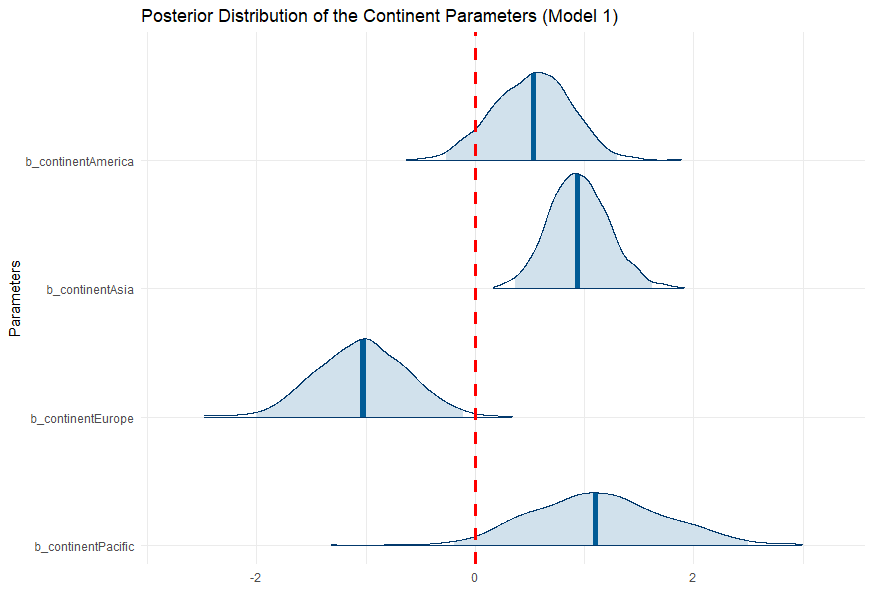
\includegraphics[scale=0.2]{PosteriorPlot_Continents_Model1.png}
\caption{Posterior Distributions $M_1$, Alliances, Border and Continents}
\end{figure}


In comparison, $M_2$ - the model without the \textit{V-Dem Index} -  indicates a similar but slightly more certain effect (see \hyperref[Appendix Tables]{\color{blue}Appendix A}) with an estimated interval of $-0.00031$ and $-0.00011$. Looking at the posterior distributions of the remaining parameters (see \hyperref[Appendix Figures]{\color{blue}Appendix B}), it is visible that excluding \textit{V-Dem} slightly shifts the estimated intervals without changing the effect signs.

\begin{figure}[h]
\center
\label{F:5}
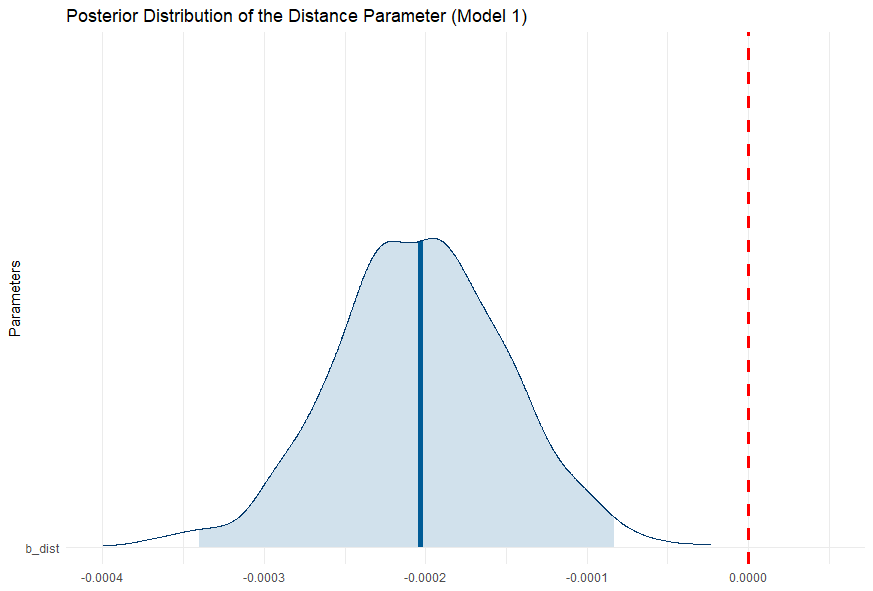
\includegraphics[scale=0.2]{PosteriorPlot_Distance_Model1.png}
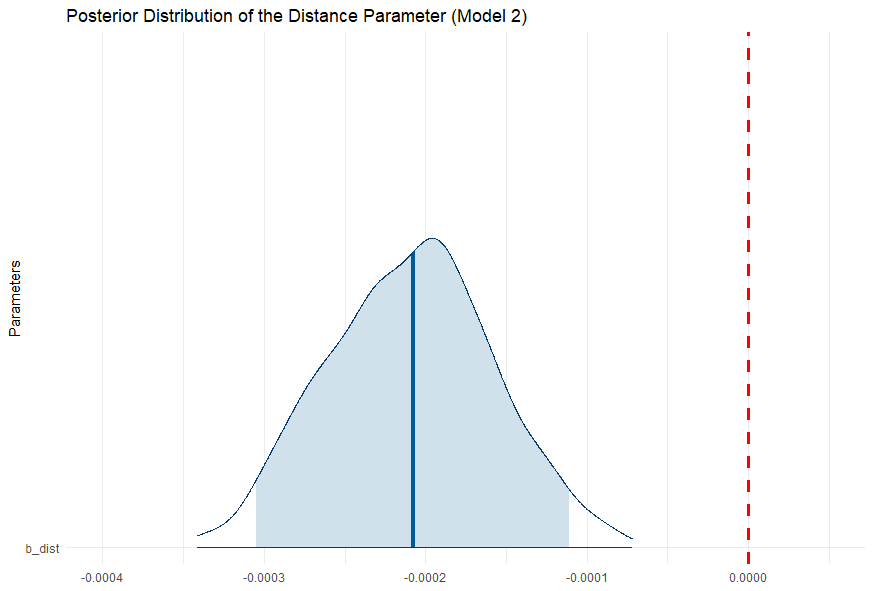
\includegraphics[scale=0.2]{PosteriorPlot_Distance_Model2.png}
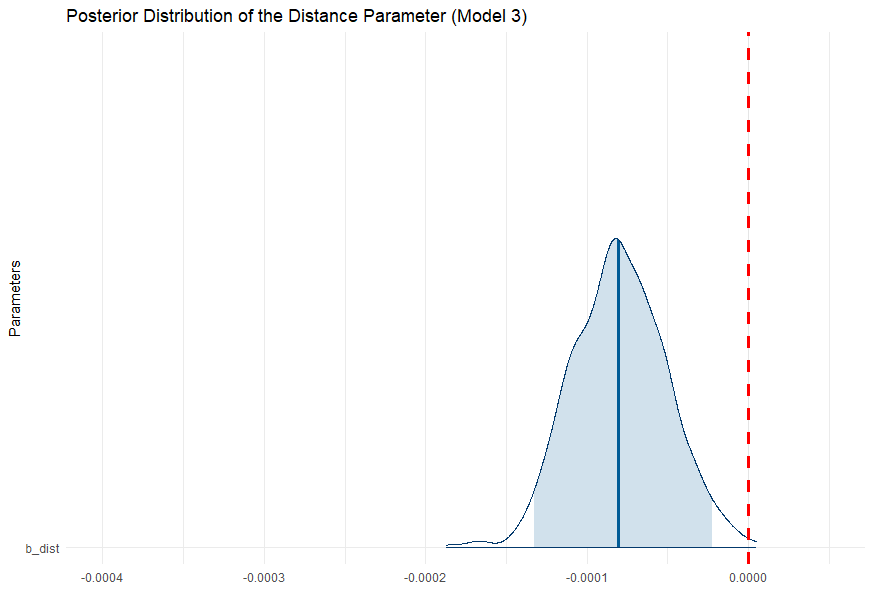
\includegraphics[scale=0.2]{PosteriorPlot_Distance_Model3.png}
\caption{Posterior Distributions $M_1$ vs. $M_2$ vs. $M_3$, Distance}
\end{figure}

Additionally, \hyperref[F:5]{\color{blue}Figure 5} visualizes the effect on \textit{Distance's} posterior distribution when excluding all covariates in $M_3$. To further extend our analysis, we computed the fourth model $M_4$, which excludes the \textit{Distance} and the \textit{V-Dem} covariates. The estimates of this model can be found in \hyperref[F:6]{\color{blue}Figure 6}. The majority of covariates show similar posterior distributions - e.g. the border covariates or the estimates related to the alliances - however, the missing effect of the excluded covariates is being absorbed by some of the estimates related to the continents. The most prominent example can be found in the distribution for the continent covariate \textit{Pacific}, which now shows a negative effect instead of the original positive one.

\begin{figure}[h]
\center
\label{F:6}
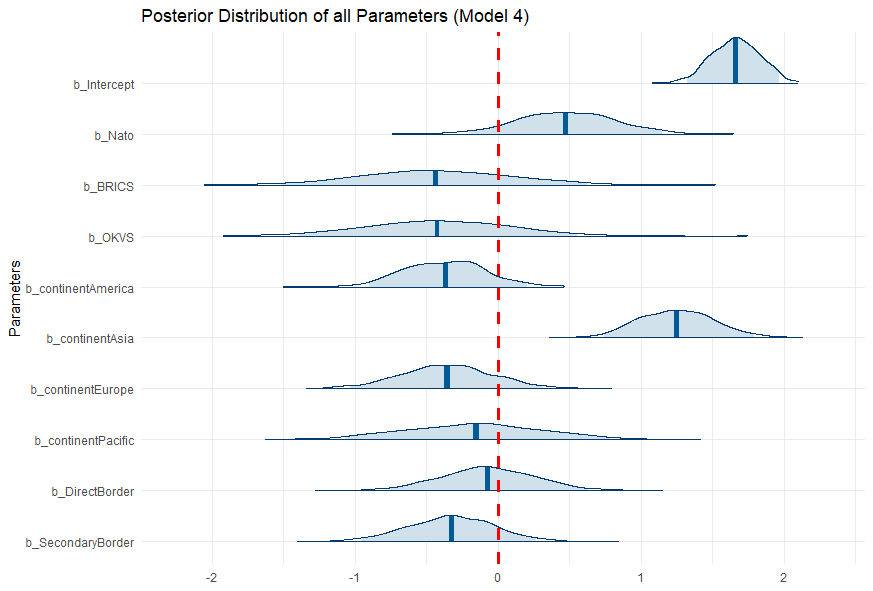
\includegraphics[scale=0.5]{PosteriorPlot_Everything_Model4NoDistnace.png}
\caption{Posterior Distributions $M_4$, every covariate}
\end{figure}


Using the Watanabe-Akaike information criterion (WAIC; introduced by \citealp{watanabe2010} as ''widely applicable information criterion''), we compute model weights as the a setup of a possible BMA approach. The computed weights can be found below in \hyperref[T:3]{\color{blue}Table 3}. We can see that the majority of the weight - more than 90\% - falls on the estimates/distributions of $M_1$. $M_3$ and $M_4$ have few to none influence on the resulting weight of the effects. As the average model prediction is dominated by $M_1$, it seems appropriate to select the first model for inference - especially since the \textit{ceteris paribus} estimated average effect only slightly differs between $M_1$ and $M_2$.
\begin{table}[!htbp] \centering 
  \caption{Estimated Model Weights} 
  \label{T:3} 
\begin{tabular}{llll}
\hline \hline
$M_1$& $M_2$ & $M_3$& $M_4$\\ \hline
0.918 & 0.082 & 0.000 & 0.000 \\ \hline \hline
\end{tabular}
\end{table}
 

\section{Discussion}
\subsection{Implications}
We fundamentally started with uncertainty across models and the different layers of distance and applied Bayesian updating of the beliefs according to the underlying data. However, given the data, a single-model selection seems after the updating more appropriate as the posterior model probability dominates the other probabilities indicating a non-arbitrariness of the model selection. While we expected a low estimated model weight on $M_3$, as it only includes one covariate, the low probability weight on the model without \textit{Distance} and \textit{V-Dem Index} supports our initial hypothesis on the capital distance's influence. \clearpage

The findings in the selected model imply that \textit{ceteris paribus} a capital city 1,000 km more distant from Moscow leads on average to a decrease of \textit{Military Expenditure in \% of GDP} by 0.2 percentage points. This effect can be seen as both statistically and economically significant, as the posterior distribution has no probability weight on zero and 0.2 percentage points represent military expenditures of a high million or low billion USD value, depending on the respective GDP. However, given the std. dev. of the military expenditure variable with 1.32, the explained variance of distance to Moscow only amounts for a fairly small share. Thus, it seems that the perceived threat of Russia is one of many determinant explaining variation in military expenditures. Still, our finding align with the findings in \citet{nordhaus2012}, as a higher perceived threat can be seen as proxy for a higher probability of war, and highlight the importance of regional distance to perceived threats as an explanation of military expenditures. 

Additionally, our findings strongly reinforce the pertinent contribution of continents in explaining the variance of military expenditures. No matter in which model, the posterior distribution of \textit{Asia} reveals a significant positive effect capturing the increasing tensions in Asia involving China. However, it is also visible in every model's posterior distribution that Europe's military expenditure are below average. Including the effect of \textit{Distance} shifts the probability mass further into the negative while increasing the certainty of the estimate, indicating a collective underestimation of the threat emanating from Russia.\footnote{For our robustness-checks we looked at different time stamps after 2000, and could interestingly see this effect increasing, even after the annexation of Crimea - see e.g. 2005 vs. 2015 in \hyperref[Appendix Tables]{\color{blue}Appendix A}.}


While we see strong evidence for the hypothesis of the geographical distance layer of distance, the results for the degree of border and sociological distance in form of the \textit{V-Dem Index} are mixed. One the one hand, the inclusions raises the predictive quality as e.g. visible in model weights, while it's also observable that the posterior distributions always include zero and, hence, should be considered a non-significant. The amount of probability mass in the realm of negative for \textit{Direct} and \textit{Secondary Border }is given the descriptive data to some extend surprising, raising questions w.r.t. the indirect conditional independence of the introduced further layers of distance. It's likely that the introduced measurements for possible allies are not able to fully capture country specific determinants. Similarly, the captured dependency between democracy and military expenditures generally highly correlates with the classification as part of a continent (as visible in \hyperref[F:2]{\color{blue}Figure 2, right panel}). Thus,  the direction of the effect must not be over-interpreted, and it should be assumed that the breakdown by continents in itself absorbs sociological differences. Nevertheless, an inclusion can be seen as optional w.r.t. to inference, as the posterior distribution of \textit{Distance} only slightly changes, and as necessary w.r.t. to raise the predictive ability. 
\subsection{Robustness \& Limitations}
Generally, our application of BMA to military expenditure data may be subject to a covariate shift, which means that the distribution of the explanatory variables may change over time or across regions. This may affect the validity and generalizability the BMA results. To control for such a covariate shift, we limit our data to the millenial era (i.e. 2000+) and do several regression for different time stamps as robustness-checks (see e.g. 2005 and 2015 in \hyperref[Appendix Tables]{\color{blue}Appendix A}).\footnote{The time-selection may seem arbitrary, but it nearly perfectly captures the considered end of the cold war \citep{gray2005}. Concerning our results, we can only assume that validity for the time frame post-Cold-War \& pre-Ukraine-Russia outbreak of war. A generalization cannot be made with certainty.} However, those regressions yield w.r.t. model weights and the \textit{Distance} covariate similar results. 
\clearpage
Furthermore, while a BME approach is normally considered a perfect approach to rule out overconfidence and the frequentist all-or-nothing mentality, we still end up with a similar result in our Bayesian approach. This leaves room of questioning our implementation of the method. It might be possible that the choice of priors for the models and the parameters may affect our posterior model probabilities and, hence, the possible model-averaged estimates. However, as we chose weakly informative priors, we unsurprisingly obverse a zero to nothing sensitivity when imposing minor changes in our priors. Additionally, we graphically assess the convergence of our MCMC-algorithm, which also ensures the validity of our results. Nevertheless, the classical BMA approach is highly dependent on the selected candidate models. We first identified possible covariates based on our hypothesis and existing literature, included the available covariates and, finally, only selected the promising models in the final consideration. Consequently, we cannot exclude biases arising from this procedure. It might be possible that we exclude the most promising model due to missing variables or missspecification. Thus, it is still possible that, since we had an extremely promising model at hand, we fell into the same trap of overconfidence as we would have done with a frequentist approach.

Additionally, we do not fully explore in this research project the possibility of using more flexible models, such as generalized additive models or Bayesian additive regression trees, which may better fit the data and reveal more complex relationships. Especially spatial models could have accounted for the spatial dependence or heterogeneity of military expenditures across countries. This might have improved our model as we observed a triangular correlation between continent, geographic and cultural distance, which we assume we have not fully absorbed. Spatial models, hence, would have offered a more realistic and flexible way to model the underlying spatial autocorrelation and heterogeneity.

Finally, the choice of data may lead to validity problems. Besides to already mentioned limitation of generalization w.r.t. time and the possible bias w.r.t. to the used electoral democracy index, especially the SIRPI database could induce validity problems, which we are not able to control for. Although the SIRPI tries to use as few secondary sources in form of estimates as possible and to validate these in retrospect, it is nevertheless necessary for us to rely completely on the data generation process. This reliability, however, is questionable, especially in terms of military data and the strategic communication of the latter. On the one hand, it may be possible that deliberate information on military spending is being whitewashed; on the other hand, a ''filter bubble bias'' could arise if the data is based on estimates that include the same covariates as we include to explain variation. A next step would be to verify our results with similar datasets, e.g. the Correlates of War (CoW) dataset.


\section{Conclusion}
Our research project contributes to the existing literature by focusing on the geographical distance to Russia as a key determinant of military spending. The novel approach in this research area of employing Bayesian Model averaging offers a robust econometric method for analyzing complex relationships that demand a high number of control variables and could be extended to further research on military expenditures. 
While our project provides strong evidence in favor of geographical distance to a possible threat being one determining factor of military expenditures, there are still several avenues for further explorations. Investigating the reasons behind specific countries’ deviations from the 2 \% GDP allocation norm within NATO and understanding how regional alliances or geopolitical interests might interact with geopolitical proximity could yield additional valuable findings. 
By utilizing measures beyond just capital city distances as a proxy for distance, our analysis reveals diverse results prompting us to consider whether further exploration with different distance definitions could contribute further to understanding this area. Moreover, a potential shift from geographical distance to political distance to Russia could still provide a fresh perspective, exploring, how countries’ political perception of Russia influences their defense spending over time.
In conclusion, our research underscores the importance of physical geography and external security factors influencing military spending decisions. By examining the influence of geographical distance to Russia on military expenditures, we have enriched our understanding of how perceived threats and security concerns are translated into defense policies on a global scale. The finding from our analysis suggest that Policymakers should consider the geographical context and security concerns when allocating defense budgets and contribute to the broader discourse on defense spending determinants, encouraging further exploration in this area.  




\clearpage


%------------------------------------------------------------------%
\pagenumbering{roman}
\setcounter{page}{\thesavepage}
\pagestyle{plain}
\addcontentsline{toc}{section}{References}
\bibliographystyle{apalike}
\bibliography{TheKremlinEffect.bib}
\clearpage
\appendix
\section{Further Tables}
\label{Appendix Tables}

\begin{table}[!htbp] \centering 
  \caption{Estimates of $M_2$, Bayesian Regression for t = 2021} 
  \label{A1} 
\begin{tabular}{@{\extracolsep{5pt}} ccccc} 
\\[-1.8ex]\hline 
\hline \\[-1.8ex] 
\textit{Military Expenditure in \% of GDP} & Estimate & Est.Error & Q2.5 & Q97.5 \\ 
\hline \\[-1.8ex] 
Intercept & $3.083$ & $0.372$ & $2.352$ & $3.805$ \\ 
Distance & $-0.0002$ & $0.0001$ & $-0.0003$ & $-0.0001$ \\ 
Nato & $0.361$ & $0.339$ & $-0.315$ & $1.038$ \\ 
BRICS & $-0.285$ & $0.511$ & $-1.237$ & $0.673$ \\ 
OKVS & $-0.759$ & $0.501$ & $-1.723$ & $0.262$ \\ 
America & $0.436$ & $0.345$ & $-0.226$ & $1.084$ \\ 
Asia & $1.013$ & $0.276$ & $0.467$ & $1.605$ \\ 
Europe & $-1.158$ & $0.376$ & $-1.921$ & $-0.416$ \\ 
Pacific & $1.089$ & $0.570$ & $-0.013$ & $2.140$ \\ 
Direct Border & $-0.366$ & $0.323$ & $-0.966$ & $0.263$ \\ 
Secondary Border & $-0.519$ & $0.297$ & $-1.101$ & $0.048$ \\ 
\hline \hline \\[-1.8ex] 
\end{tabular} 
\end{table} 

\vfill


\begin{table}[!htbp] \centering 
  \caption{Estimates of $M_1$, Bayesian Regression for t = 2005} 
  \label{A2} 
\begin{tabular}{@{\extracolsep{5pt}} ccccc} 
\\[-1.8ex]\hline 
\hline \\[-1.8ex] 
 \textit{Military Expenditure in \% of GDP}& Estimate & Est.Error & Q2.5 & Q97.5 \\ 
\hline \\[-1.8ex] 
Intercept & $3.099$ & $0.377$ & $2.363$ & $3.831$ \\ 
Distance & $-0.0002$ & $0.0001$ & $$-$0.0003$ & $$-$0.0001$ \\ 
Nato & $0.474$ & $0.344$ & $$-$0.210$ & $1.144$ \\ 
BRICS & $0.046$ & $0.524$ & $$-$1.044$ & $1.018$ \\ 
OKVS & $$-$0.685$ & $0.510$ & $$-$1.741$ & $0.274$ \\ 
America & $0.586$ & $0.370$ & $$-$0.123$ & $1.333$ \\ 
Asia & $1.057$ & $0.253$ & $0.583$ & $1.560$ \\ 
Europe & $$-$0.694$ & $0.419$ & $$-$1.510$ & $0.133$ \\ 
Pacific & $0.914$ & $0.557$ & $$-$0.183$ & $2.008$ \\ 
Direct Border & $$-$0.534$ & $0.314$ & $$-$1.142$ & $0.078$ \\ 
Secondary Border & $$-$0.503$ & $0.287$ & $$-$1.038$ & $0.087$ \\ 
V-Dem Index & $$-$0.756$ & $0.445$ & $$-$1.627$ & $0.104$ \\ 
\hline \hline \\[-1.8ex] 
\end{tabular} 
\end{table} 
\vfill 
\begin{table}[t] \centering 
  \caption{Estimates of $M_1$, Bayesian Regression for t = 2015} 
  \label{A3} 
\begin{tabular}{@{\extracolsep{5pt}} ccccc} 
\\[-1.8ex]\hline 
\hline \\[-1.8ex] 
 \textit{Military Expenditure in \% of GDP}& Estimate & Est.Error & Q2.5 & Q97.5 \\ 
\hline \\[-1.8ex] 
Intercept & $3.460$ & $0.477$ & $2.523$ & $4.401$ \\ 
Distance & $$-$0.0002$ & $0.0001$ & $$-$0.0003$ & $$-$0.0001$ \\ 
Nato & $0.220$ & $0.417$ & $$-$0.561$ & $1.008$ \\ 
BRICS & $$-$0.218$ & $0.576$ & $$-$1.412$ & $0.913$ \\ 
OKVS & $$-$0.539$ & $0.599$ & $$-$1.680$ & $0.618$ \\ 
America & $0.704$ & $0.402$ & $$-$0.058$ & $1.515$ \\ 
Asia & $1.408$ & $0.339$ & $0.746$ & $2.079$ \\ 
Europe & $$-$0.917$ & $0.462$ & $$-$1.811$ & $0.021$ \\ 
Pacific & $1.016$ & $0.669$ & $$-$0.267$ & $2.316$ \\ 
Direct Border & $-0.307$ & $0.382$ & $-1.022$ & $0.438$ \\ 
Secondary Border & $-0.768$ & $0.350$ & $$-$1.501$ & $$-$0.085$ \\ 
V-Dem Index & $-0.983$ & $0.530$ & $$-$2.004$ & $0.097$ \\ 
\hline \hline \\[-1.8ex] 
\end{tabular} 
\end{table} 
\vfill
 \clearpage
\section{Further Figures}
\label{Appendix Figures}
\begin{figure}[h]
\center
\label{F:B1}
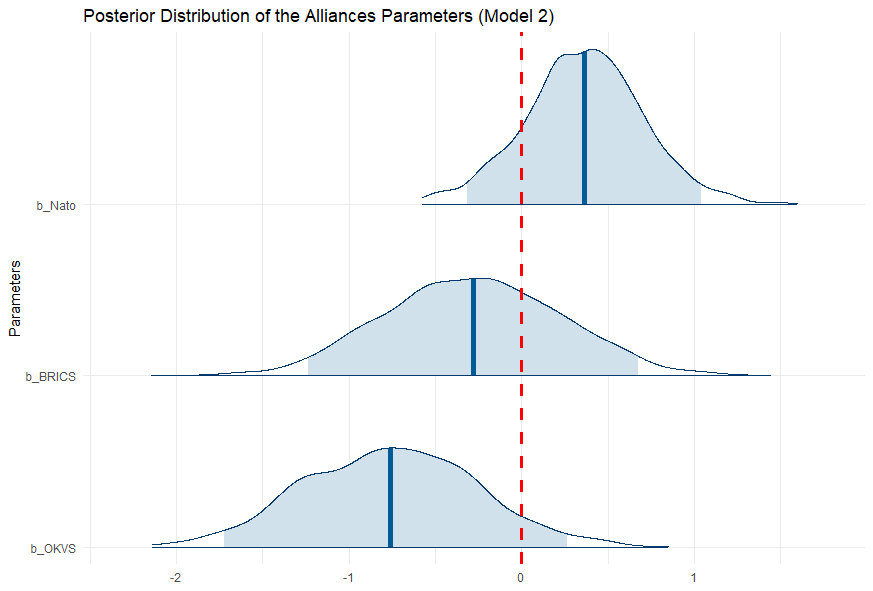
\includegraphics[scale=0.3]{PosteriorPlot_Alliances_Model2.png}
\caption{Posterior Distributions $M_2$, Alliances}
\end{figure}
\vfill
\begin{figure}[h]
\center
\label{F:B2}
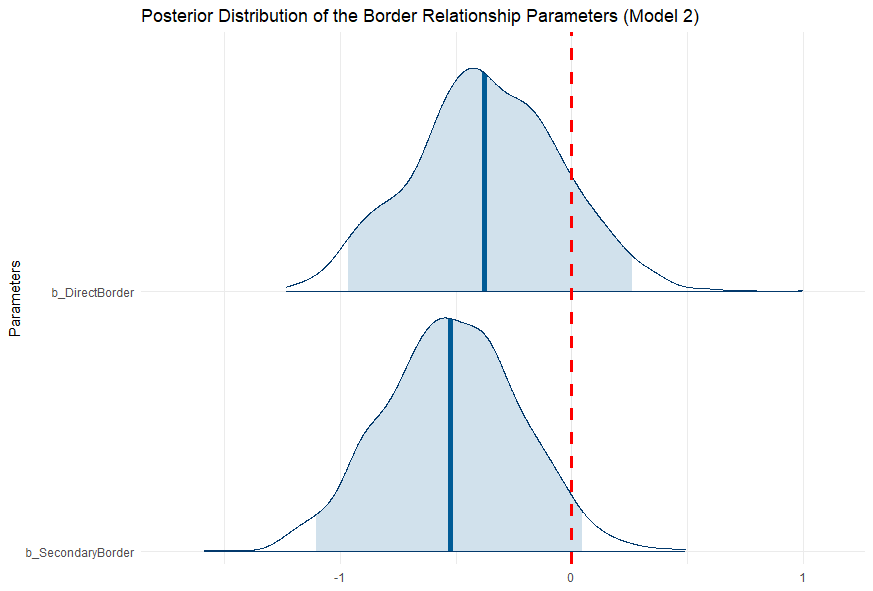
\includegraphics[scale=0.3]{PosteriorPlot_Border_Model2.png}
\caption{Posterior Distributions $M_2$, Border}
\end{figure}
\vfill
\begin{figure}[h]
\center
\label{F:B3}
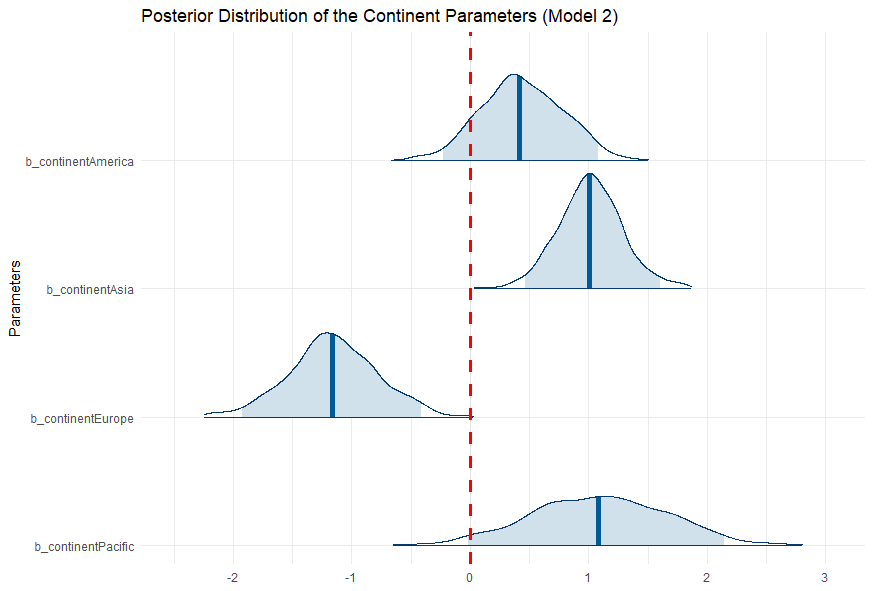
\includegraphics[scale=0.3]{PosteriorPlot_Continents_Model2.png}
\caption{Posterior Distributions $M_2$, Continents}
\end{figure}

\vfill



\end{document}
